\section{Auswertung}
\label{sec:Auswertung}

\subsection{Bestimmung der Magnetischen Flussdichte von zwei Spulen unterschiedlicher Länge}
In Tabelle (1) befinden sich die Messwerte der magnetischen Flussdichte $B$ für einer kurzen Spule und in Tabelle (2) die der großen Spule.
Diese sind in Abhängigkeit vom Abstand $x$ in Abbildung (6) und (7) graphisch dargestellt.
Beide Spulen befinden sich rechts des Ursprungs und beginnen bei diesem.

%tabkurz&lang
\begin{minipage}{0.5\textwidth}
\begin{table}[H]
  \centering
  \caption{Magnetische Flussdichte $B$ \\ und Abstand $x$ einer kurzen Spule.}
  \begin{tabular}{c c}
    \toprule
     $x/$cm & $B/$mT  \\
    \midrule
    -5 & 0,039 \\
    -4 & 0,079 \\
    -3 & 0,147 \\
    -2 & 0,287 \\
    -1 & 0,567 \\
    0 & 1,130\\
    1 & 1,551 \\
    2 & 1,801 \\
    3 & 1,838 \\
    4 & 1,684 \\
    5 & 1,351 \\
    6 & 0,728 \\
    7 & 0,377 \\
    8 & 0,173 \\
    9 & 0,100 \\
    10 & 0,060 \\
    11 & 0,035 \\
    12 & 0,018 \\
  \bottomrule
  \end{tabular}
\end{table}
\end{minipage}
\begin{minipage}{0.5\textwidth}
\begin{table}[H]
  \centering
  \caption{Magnetische Flussdichte $B$ \\ und Abstand $x$ einer langen Spule.}
  \begin{tabular}{c c}
    \toprule
     $x/$cm & $B/$mT  \\
    \midrule
    - & - \\
    -4 & 0,131 \\
    -3 & 0,193 \\
    -2 & 0,316 \\
    -1 & 0,569 \\
    0 & 1,033\\
    1 & 1,648 \\
    2 & 2,007 \\
    3 & 2,185 \\
    4 & 2,280 \\
    5 & 2,330 \\
    6 & 2,353 \\
    7 & 2,369 \\
    8 & 2,374 \\
    9 & 2,372 \\
    10 & 2,364 \\
    11 & 2,346 \\
    12 & 2,307 \\
  \bottomrule
  \end{tabular}
\end{table}
\end{minipage}
\\~\\

Als experimentell bestimmte Flussdichte $B_\text{XX, exp}$ wird jeweils das Maximum der Messreihe gewählt.
Die theoretische Flussdichte $B_\text{XX, th}$ wird mit Gleichung (1) bestimmt.
So ergibt sich für die kurze Spule eine Flussdichte von 
\begin{align*}
B_\text{KS, exp} = 1,838\,\si{\milli\tesla}
\end{align*}
und
\begin{align*}
B_\text{KS, th} = 2,055\,\si{\milli\tesla}.
\end{align*}

Für die lange Spule ergibt sich eine Flussdichte von 
\begin{align*}
B_\text{LS, exp} = 2,374\,\si{\milli\tesla}
\end{align*}
und
\begin{align*}
B_\text{LS, th} = 2,424\,\si{\milli\tesla}.
\end{align*}

%PLOTKURZ
\begin{figure}[H]
  \centering
  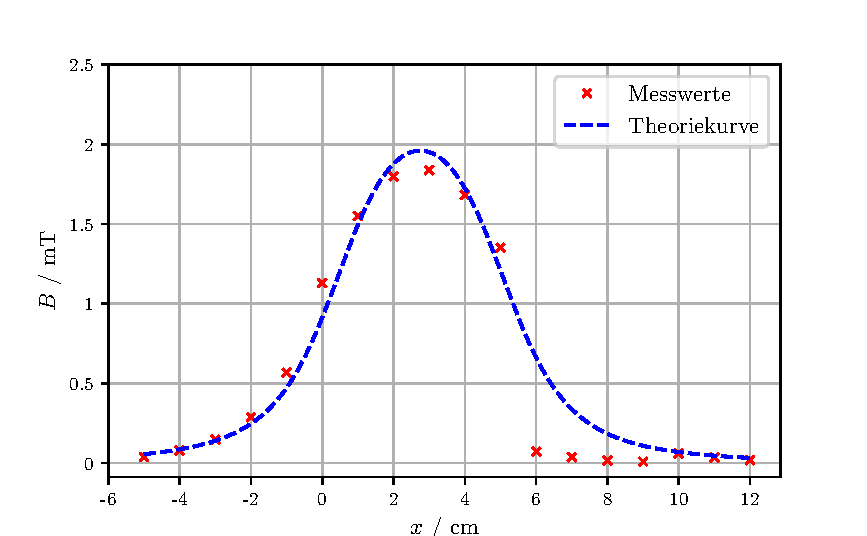
\includegraphics{kurz.pdf}
  \caption{Magnetische Flussdichte $B$ einer kurzen Spule.}
  \label{fig:plot}
\end{figure}
%PLOTLANG
\begin{figure}[H]
  \centering
  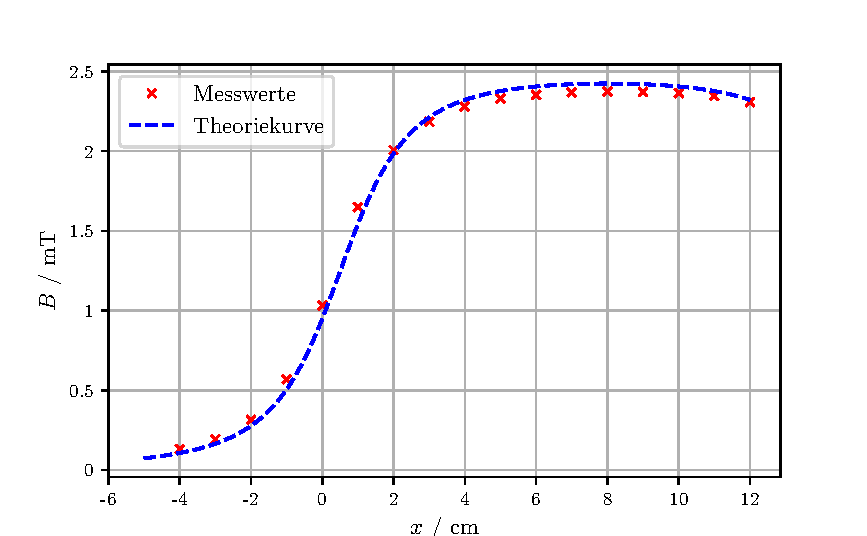
\includegraphics{lang.pdf}
  \caption{Magnetische Flussdichte $B$ einer langen Spule.}
  \label{fig:plot}
\end{figure}

%HELMHOLTZ
\subsection{Bestimmung der Magnetischen Flussdichte eines Helmholtzspulenpaares}
Die magnetische Flussdichte in der Mitte eines Helmholtzspulenpaares wird für den Abstand 
des Eigendurchmessers $d$ = 12,5cm mit der Stromstärke $I$ = 2 A und 4 A und des 
Eigenradius $r$ = 6,25cm mit der Stromstärke $I$ = 2 A gemessen.
Die Messwerte befinden sich in Tabelle (3), (4) und (5). Die ersten zwei Messungen sind in
Abbildung (8) dargestellt, die letzte in Abbildung (9).

%TABHELMHOLTZ
\begin{minipage}{0.6\textwidth}
\begin{table}[H]
  \centering
  \caption{Magnetische Flussdichte $B$ und \\ Abstand $x$ des Helmholtzspulenpaares \\ im Abstand $d$ = 12,5 cm, \\ bei $I$ = 2 A.}
  \begin{tabular}{c c}
    \toprule
     $x/$cm & $B/$mT  \\
    \midrule
    3 & 1,700 \\
    4 & 1,565 \\
    5 & 1,470 \\
    6 & 1,435 \\
    7 & 1,466 \\
    8 & 1,557\\
    9 & 1,694 \\
    15 & 1,541 \\
    16& 1,281\\
    17& 1,031 \\
    18& 0,808 \\
    19& 0,633 \\
  \bottomrule
  \end{tabular}
\end{table}
\end{minipage}
\begin{minipage}{0.6\textwidth}
\begin{table}[H]
  \centering
  \caption{Magnetische Flussdichte $B$  und \\ Abstand $x$ des Helmholtzspulenpaares \\ im Abstand $d$ = 12,5 cm, \\ bei $I$ = 4 A.}
  \begin{tabular}{c c}
    \toprule
     $x/$cm & $B/$mT  \\
    \midrule
    3 & 3,515 \\
    4 & 3,258 \\
    5 & 3,074 \\
    6 & 3,004 \\
    7 & 3,073 \\
    8 & 3,255\\
    9 & 3,235 \\
    15 & 3,256 \\
    16& 2,761 \\
    17& 2,786 \\
    18& 1,865 \\
    19& 1,506 \\
  \bottomrule
  \end{tabular}
\end{table}
\end{minipage}
%TABHELMHOLTZ2
\begin{table}[H]
  \centering
  \caption{Magnetische Flussdichte $B$  und Abstand $x$ des Helmholtzspulenpaares  im Abstand $r$ = 6,25 cm, bei $I$ = 2 A.}
  \begin{tabular}{c c}
    \toprule
     $x/$cm & $B/$mT  \\
    \midrule
    2,8 & 2,724 \\
    2,9 & 2,728 \\
    3,0 & 2,729 \\
    3,1 & 2,729 \\
    3,2 & 2,729 \\
    3,3 & 2,729 \\
    3,4 & 2,728 \\
    9 & 1,380\\
    10 & 1,460 \\
    11 & 1,170 \\
    12 & 0,901 \\
    13 & 0,701 \\
    14 & 0,544 \\

   
  \bottomrule
  \end{tabular}
\end{table}

Für den experimentell bestimmten Wert der magnetischen Flussdichte in der Mitte des 
Spulenpaares wird im Fall, dass
der Abstand zwischen dem Spulenpaar dem Eigendurchmesser entspricht, der Wert im Tiefpunkt
des Graphen, also bei $x$ = 6 cm gewählt und ergibt sich so zu
\begin{align*}
B_\text{Hd2A, exp} = 1,435\,\si{\milli\tesla}
\end{align*}
und
\begin{align*}
B_\text{Hd4A, exp} = 3,004\,\si{\milli\tesla}.
\end{align*}

Entspricht der Abstand zwischen dem Spulenpaar dem Eigenradius, so wird der Messwert bei
$x$ = 3,1 cm als magnetische Flussdichte in der Mitte des Spulenpaares gewählt und ergibt sich
zu
\begin{align*}
B_\text{Hr, exp} = 2,729\,\si{\milli\tesla}.
\end{align*}

Die entsprechenden theoretischen Werte werden mittels Gleichung (4) zu
\begin{align*}
B_\text{Hd2A, th} &=  1,637\,\si{\milli\tesla}\\
B_\text{Hd4A, th} &=  3,274\,\si{\milli\tesla}\\
B_\text{Hr, th} &= 2,877\,\si{\milli\tesla}
\end{align*}
bestimmt.

\begin{figure}[H]
  \centering
  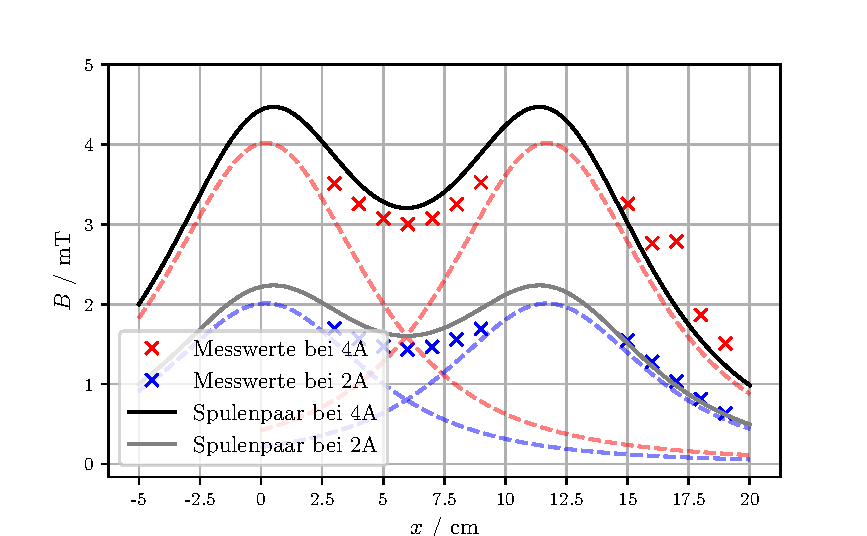
\includegraphics{helmholtzD.pdf}
  \caption{Magnetische Flussdichte $B$ eines Helmholtzspulenpaares im Abstand des Durchmessers $d$ = 12,5 cm.}
  \label{fig:plot}
\end{figure}

\begin{figure}[H]
  \centering
  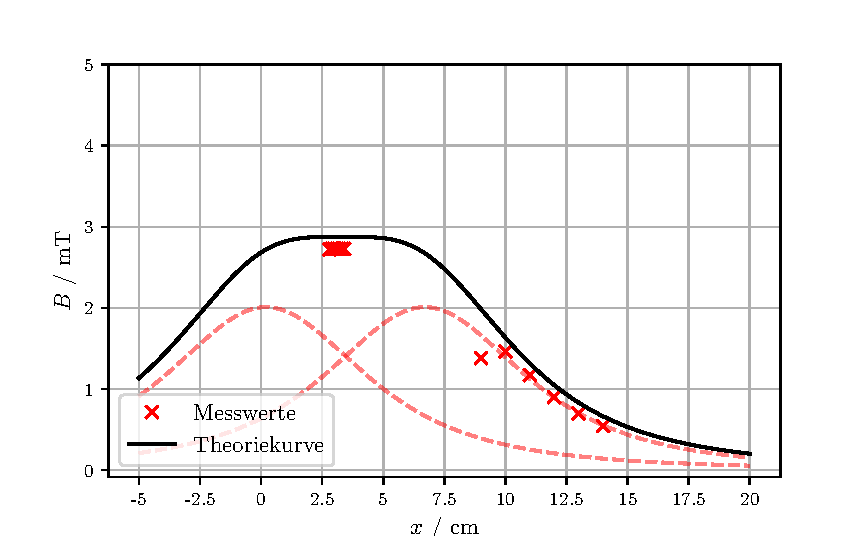
\includegraphics{helmholtzR.pdf}
  \caption{Magnetische Flussdichte $B$ eines Helmholtzspulenpaares im Abstand des Radius $r$ =\,6,25 cm.}
  \label{fig:plot}
\end{figure}


\subsection{Bestimmung einer Hysteresekurve eines Eisenkerns mit Luftspalt in einer Toroidspule.}
Die Messwerte der magnetischen Flussdichte in Abhängigkeit der Stromstärke $I$
für die Hysteresekurve sind in der Tabelle (6) zu finden. Mittels Gleichung (2) lässt sich aus
der Stromstärke die magnetische Feldstärke $H$ bestimmen, in dessen Abhängigkeit die magnetische
Flussdichte $B$ in Abbildung (10) aufgetragen wird.\\
Aus dieser wird nun die Sättigungsmagnetisierung $B_\text{s}$, die Remanenz $B_\text{r}$ und 
die Koerzitivkraft $H_\text{c}$ abgelesen:
\begin{align*}
B_\text{s} &= 688,8\,\si{\milli\tesla},\\
B_\text{r} &= 122,2\,\si{\milli\tesla},\\
H_\text{c} &= 457,4\,\si{\ampere\per\meter}.
\end{align*}

\begin{figure}[H]
  \centering
  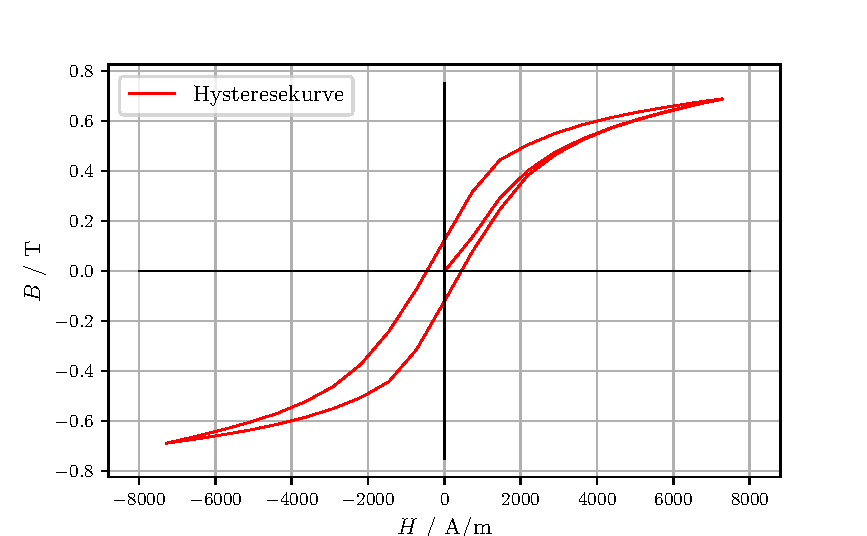
\includegraphics{plothyst.pdf}
  \caption{Hysteresekurve eines Eisenkerns mit Luftspalt in einer Toroidspule.}
  \label{fig:plot}
\end{figure}


\begin{table}[H]
  \centering
  \caption{Magnetische Flussdichte und Stromstärke einer Ringspule.}
  \begin{tabular}{c c | c c | c c | c c | c c}
    \toprule
     $I/A$ & $B/mT$ &$I/A$ & $B/mT$ & $I/A$ & $B/mT$ &$I/A$ & $B/mT$ & $I/A$ & $B/mT$  \\
    \midrule
    0 &-2,562 & 9 & 673,6 & -1 & -0,724 & -9 & -673,9 & 1 & 75,66\\
    1 & 134,2 & 8 & 655,7 & -2 & -242,8 & -8 & -656,0 & 2 & 246,5\\
    2 & 292,3 & 7 & 636,5 & -3 & -373,8 & -7 & -636,9 & 3 & 382,7\\
    3 & 401,1 & 6 & 613,7 & -4 & -463,2 & -6 & -613,8 & 4 & 466,1\\
    4 & 476,5 & 5 & 585,8 & -5 & -523,2 & -5 & -585,6 & 5 & 525,7\\
    5 & 529,8 & 4 & 551,0 & -6 & -569,5 & -4 & -551,1 & 6 & 571,6\\
    6 & 573,2 & 3 & 504,7 & -7 & -605,5 & -3 & -506,6 & 7 & 606,3\\
    7 & 608,4 & 2 & 444,3 & -8 & -636,5 & -2 & -443,6 & 8 & 636,5\\
    8 & 638,4 & 1 & 315,1 & -9 & -664,2 & -1 & -314,6 & 9 & 664,0\\
    9 & 664,8 & 0 & 122,2 & -10 & -689,4 & 0 & -122,0 & 10 & 687,5\\
    10 & 688,8 \\
   
    
  \bottomrule
  \end{tabular}
\end{table}

